\section{Schedule}{\label{secSched}

As of March 2025, the LSSTCam is being installed on the telescope. By the first half of April, it should be pumped down and cold with initial functional checks complete. It is expected LSSTCam and the Rubin Observatory will go on sky for the first time in mid April 2025. Figure~\ref{sched} shows the current milestones for the Project and Operations.

\begin{figure}%[]
  \centering
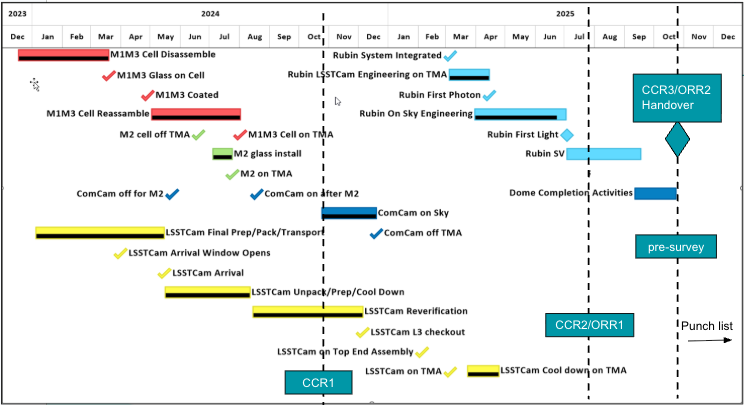
\includegraphics[width=0.95\linewidth]{sched.png}
\caption{Rubin Observatory Schedule as of late February, 2025. The forecast puts the system on sky by mid April. Planning for success, the handover to Operations is planned for early September and the start of the survey by November. Formal completeness reviews including operations readiness are shown in the Figure and described in Figure~\ref{ccr}. }
\label{sched}
\end{figure}

\newpage

The Project will complete with several reviews as described in Figure~\ref{ccr}. The first of these, Construction Completeness Review (CCR) 1, was held in October, 2024. The main review, for substantial completion and validation of system and science requirements, CCR2, is programed for late July, 2025. Concurrent to CCR2, the Operations team will go through the Operations Readiness Review (ORR) 1. At this review, the Operations team will demonstrate they are ready for handover. That is, to assume authority and responsibility for running Rubin Observatory as a system. At CCR3, any final punch list items from the Project will be verified and for ORR2, the Operations team will present the schedule for starting the LSST; i.e., the status of the system with respect to the criteria enumerated in this document.  

\begin{figure}%[]
  \centering
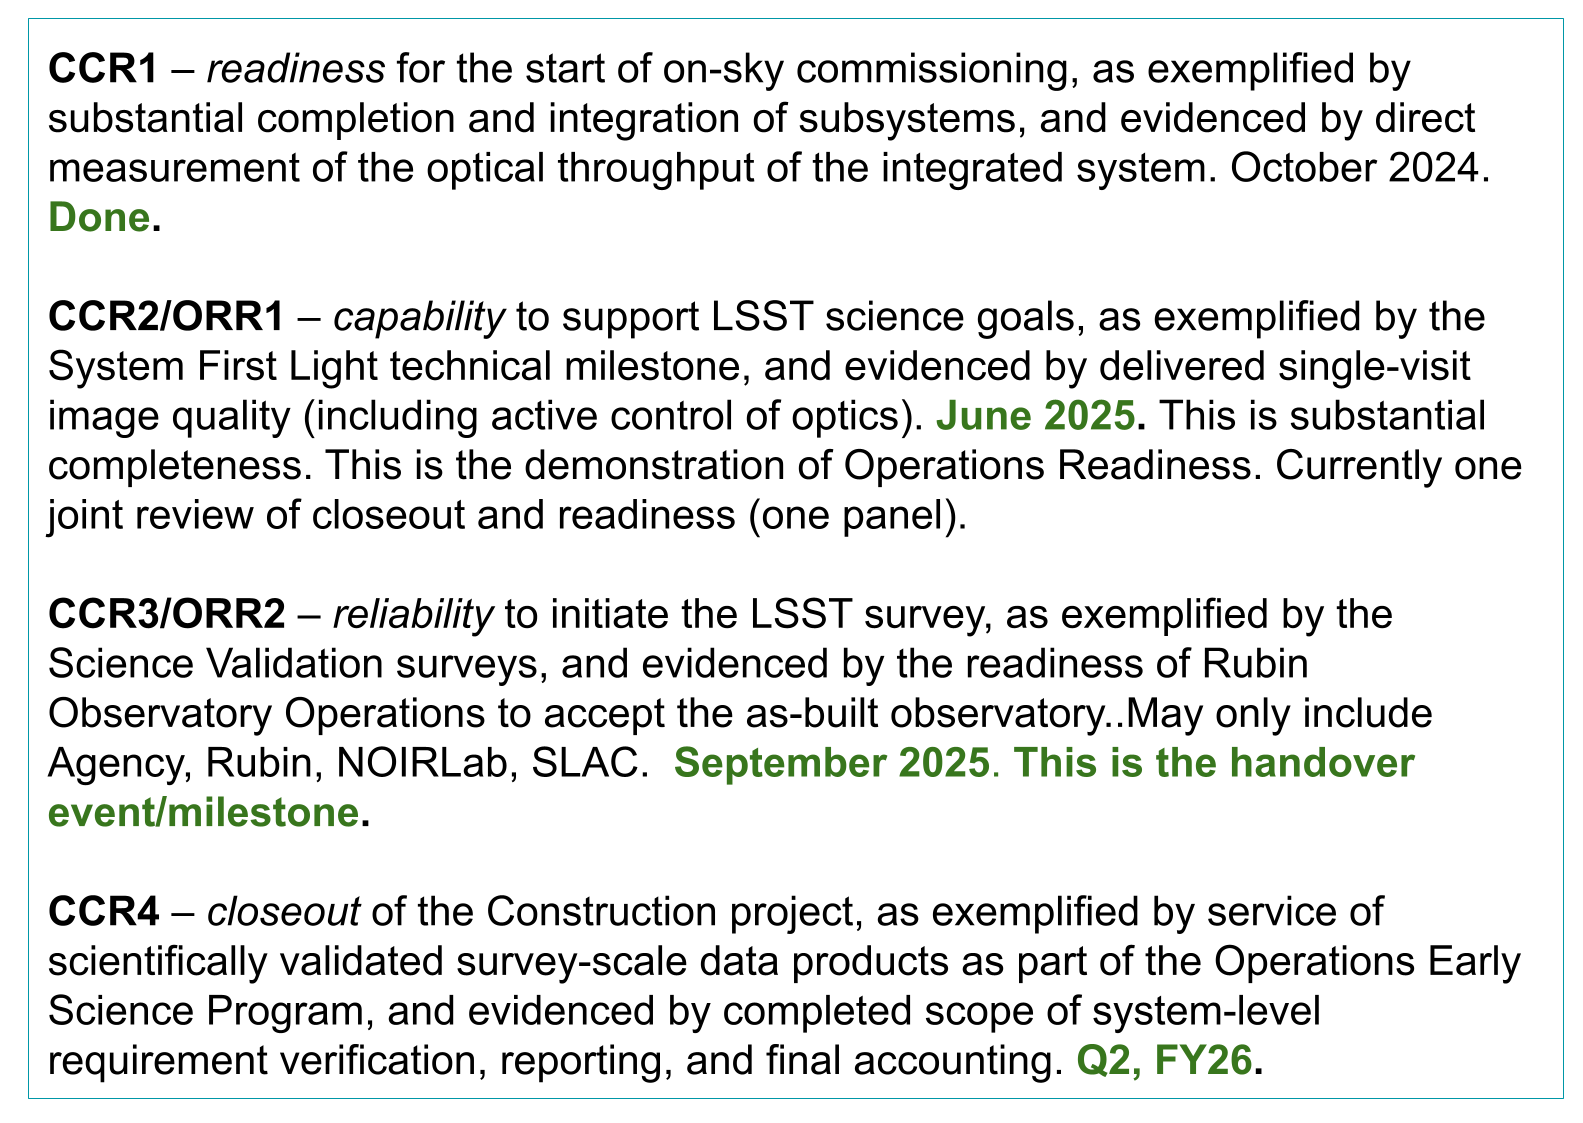
\includegraphics[width=0.65\linewidth]{ccr.png}
\caption{Construction Completeness Reviews (CCR) and concurrent Operations Readiness Reviews. CCR1-3 and ORR1-2 are required before the handover and start of LSST. CCR4 is an administrative $''$review$''.$ All CCRs and ORRs are convened by NSF and DOE.}
\label{ccr}
\end{figure}

\newpage
